\documentclass[12pt]{article}

\usepackage{sbc-template}
\usepackage[utf8]{inputenc}
\usepackage[brazil]{babel}
\usepackage{graphicx}
\usepackage{url}
\usepackage{amsmath}
\usepackage{array}

\sloppy

\title{Poluicao Luminosa na Costa de Santa Catarina: um Pipeline de Processamento de Imagem para Estimar Risco Ecologico Relativo}

\author{Pedro Pacheco\inst{1}, Carlos Soler\inst{1}}

\address{Universidade Regional de Blumenau (FURB)\\
Disciplina de Processamento de Imagem}

\begin{document}

\maketitle

\begin{abstract}
This paper presents an image-processing workflow for investigating artificial night light near aquatic environments on the coast of Santa Catarina, Brazil. The study focuses on Florianopolis, Balneario Camboriu and Itajai. Instead of training a supervised neural network, the work implements a deterministic classification pipeline that combines water segmentation, VIIRS night-light layers, marine buffers, productivity proxies, fauna sensitivity and protected-area overlays. The output is a relative ecological-risk index designed for comparison between cities and for visual interpretation in an image-processing course context.
\end{abstract}

\begin{resumo}
Este artigo apresenta um fluxo de processamento de imagem para investigar a presenca de luz artificial noturna proxima a ambientes aquaticos na costa de Santa Catarina. O estudo considera Florianopolis, Balneario Camboriu e Itajai. Em vez de treinar uma rede neural supervisionada, foi implementado um classificador deterministico que combina segmentacao de agua, camadas de luz noturna VIIRS, buffers marinhos, proxies de produtividade, sensibilidade de fauna e sobreposicao com unidades de conservacao. O resultado e um indice ecologico relativo, voltado a comparacao entre cidades e a interpretacao visual dentro do contexto da disciplina de Processamento de Imagem.
\end{resumo}

\section{Introducao}

A luz artificial noturna e um indicador visual de urbanizacao, infraestrutura, portos, turismo e ocupacao costeira. Em regioes litoraneas, essa iluminacao pode alcancar praias, rios, canais, estuarios e baiais, alterando condicoes naturais de orientacao, alimentacao, reproducao e migracao de organismos aquaticos e costeiros. O problema e especialmente relevante em areas urbanizadas de Santa Catarina, onde cidades costeiras combinam crescimento urbano, atividades portuarias e intensa ocupacao turistica.

O objetivo deste trabalho e desenvolver um pipeline de processamento de imagem capaz de identificar e comparar a exposicao luminosa sobre areas de agua em Florianopolis, Balneario Camboriu e Itajai. A partir dessa exposicao, o trabalho constroi uma camada adicional de risco ecologico relativo. O indice nao pretende provar impacto biologico direto; seu papel e organizar evidencias espaciais em uma escala comparavel, permitindo discutir onde luz, agua, produtividade, sensibilidade de fauna e unidades de conservacao coincidem.

A proposta foi implementada como uma arquitetura modular de classificacao por imagem. Embora o enunciado da atividade mencionasse TensorFlow, Keras ou scikit-learn, a base disponivel nao possuia rotulos supervisionados confiaveis para treinamento de uma rede neural. Por isso, adotou-se uma abordagem deterministica, auditavel e coerente com sensoriamento remoto: segmentacao por indice espectral, normalizacao de radiancia, classificacao por buffers e combinacao ponderada de camadas ambientais.

\section{Desenvolvimento e Descricao do Problema}

\subsection{Problema a ser resolvido}

O problema pode ser descrito como uma classificacao espacial: dado um conjunto de imagens e camadas derivadas, identificar regioes aquaticas que estao proximas de luz artificial noturna e estimar um risco relativo para ambientes costeiros. A pergunta central e: entre as cidades analisadas, onde a iluminacao artificial se sobrepoe a agua costeira e a proxies de sensibilidade ecologica?

A saida esperada nao e uma classe biologica absoluta, mas uma representacao comparavel entre cidades. O indice final combina exposicao luminosa, presenca/sensibilidade de fauna, produtividade primaria e habitat raso:

\[
risco = luz\_fundo \times habitat \times fauna
\]

Essa equacao foi implementada em escala normalizada entre 0 e 1. Valores mais altos indicam maior coincidencia espacial entre luz artificial, agua rasa/produtiva e grupos biologicos sensiveis.

\subsection{Montagem da base}

A base foi montada a partir de imagens de referencia diurnas e noturnas, mascaras de agua, mapas de radiancia sobre agua e camadas ambientais derivadas. As tres cidades foram processadas de forma padronizada, mantendo o mesmo raio de recorte e a mesma logica de geracao de imagens.

\begin{figure}[ht]
\centering
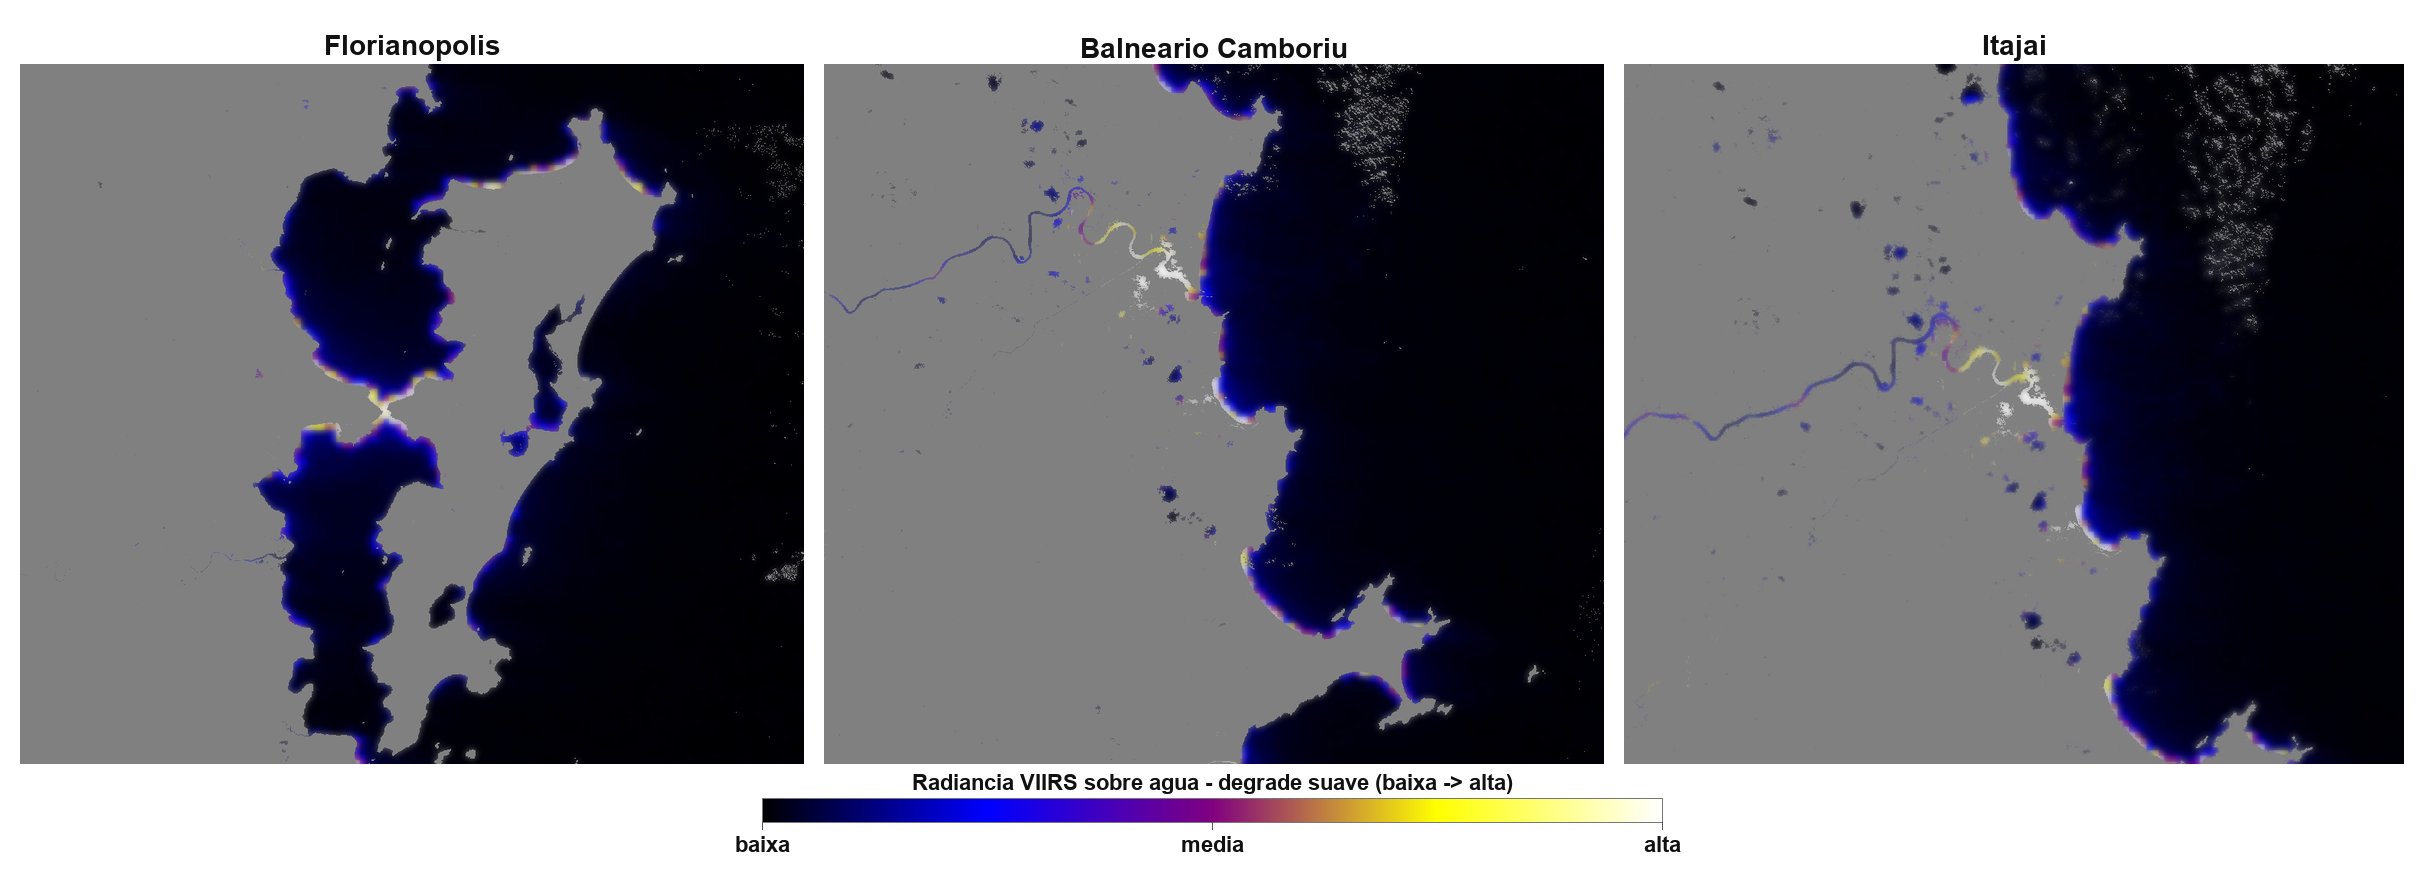
\includegraphics[width=0.95\textwidth]{../Images/comparisons/comparison-cities-smooth-gradient.png}
\caption{Comparacao visual entre as tres cidades usando gradiente suavizado de exposicao luminosa sobre agua. A figura contextualiza a diferenca espacial entre baiais, orlas urbanizadas e area portuaria.}
\label{fig:smooth}
\end{figure}

Os principais insumos do projeto sao:
\begin{itemize}
  \item imagens Sentinel-2 para separacao agua/terra por MNDWI;
  \item imagens VIIRS/Black Marble ou camadas equivalentes para luz noturna;
  \item imagens intermediarias do proprio projeto, como mascaras de agua e gradientes de exposicao;
  \item pesos de fauna derivados de OBIS com fallback AquaMaps;
  \item camada de produtividade primaria, baseada em clorofila-a quando disponivel ou em fallback local reprodutivel;
  \item catalogo de unidades de conservacao em CSV, com suporte a GeoJSON externo.
\end{itemize}

\subsection{Preparacao e pre-processamento}

O primeiro passo foi separar agua e terra. O script \texttt{water\_land\_separation.py} gera visualizacoes MNDWI e mascaras binarias. A agua e representada em verde/azul na mascara, enquanto pixels fora da agua sao tratados como fundo.

\begin{figure}[ht]
\centering
\begin{minipage}{0.32\textwidth}
\centering
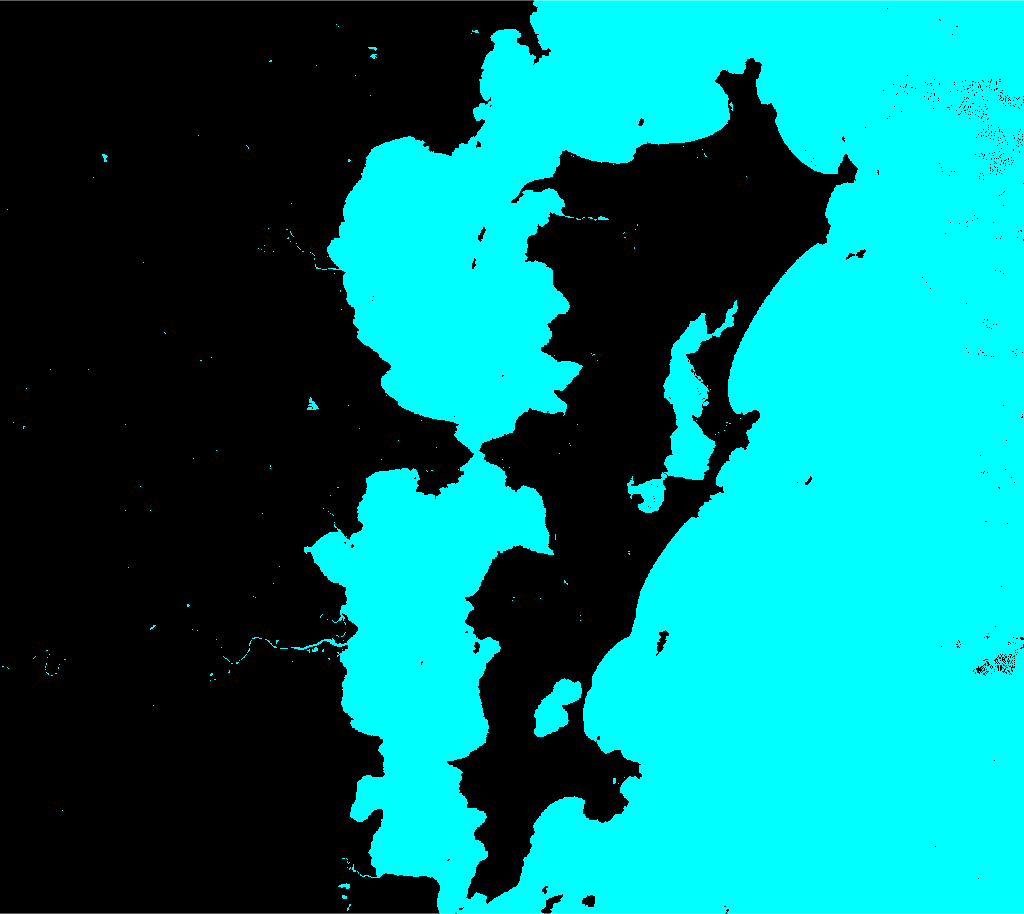
\includegraphics[width=\textwidth]{../Images/water-masks/florianopolis-water-mask.png}\\
{\small Florianopolis}
\end{minipage}
\begin{minipage}{0.32\textwidth}
\centering
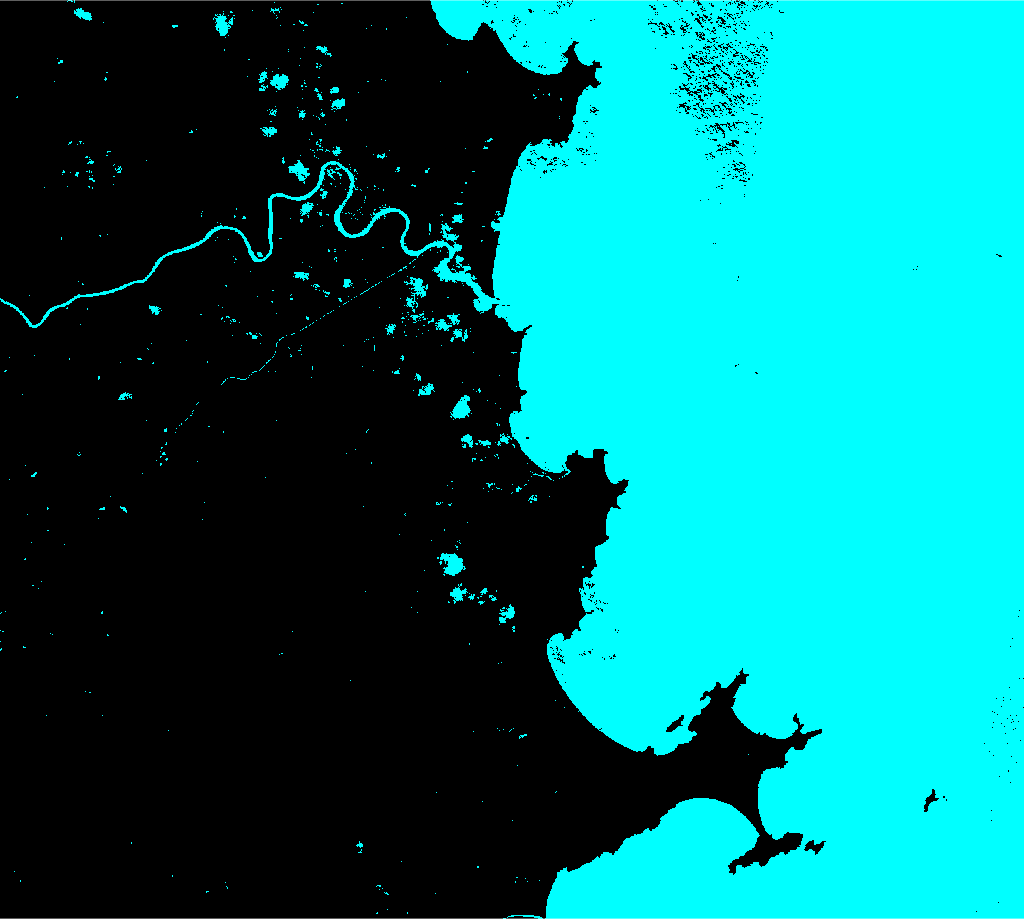
\includegraphics[width=\textwidth]{../Images/water-masks/balneario-camboriu-water-mask.png}\\
{\small Balneario Camboriu}
\end{minipage}
\begin{minipage}{0.32\textwidth}
\centering
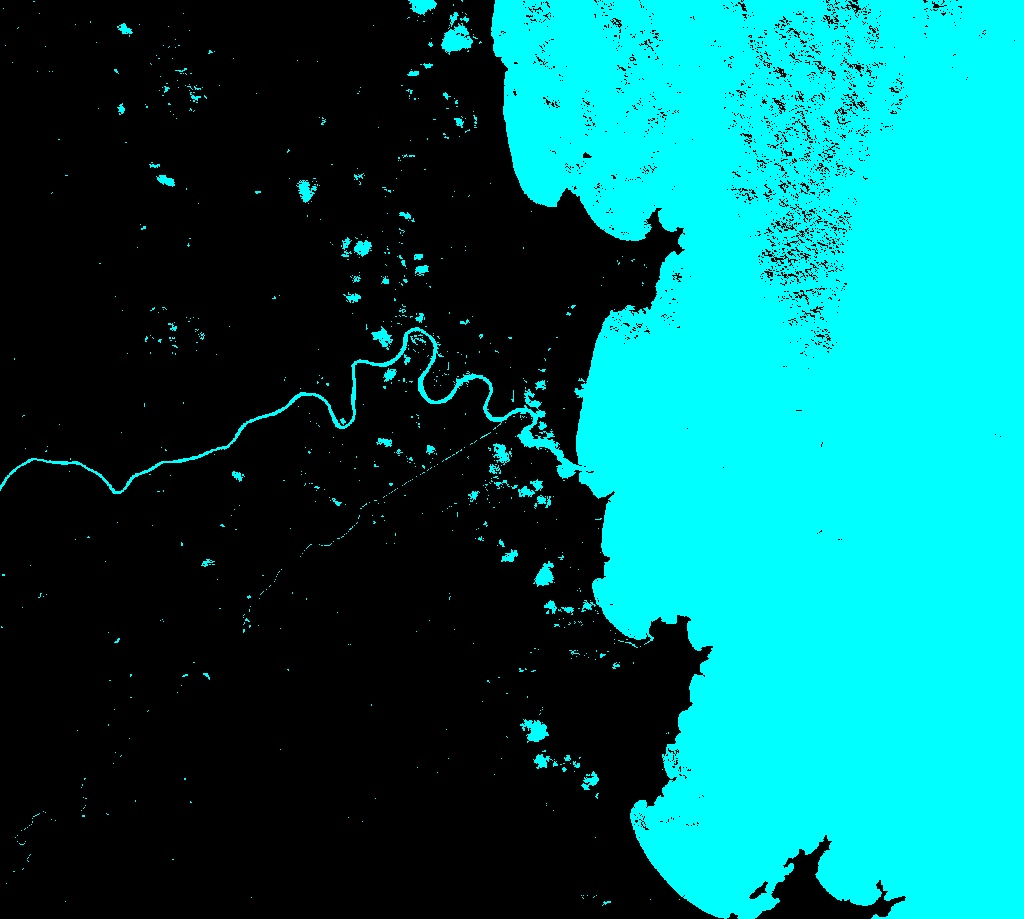
\includegraphics[width=\textwidth]{../Images/water-masks/itajai-water-mask.png}\\
{\small Itajai}
\end{minipage}
\caption{Mascaras de agua usadas como base espacial para restringir a analise aos ambientes aquaticos. Essa etapa evita interpretar luz sobre area urbana como exposicao direta da agua.}
\label{fig:masks}
\end{figure}

Em seguida, os scripts de exposicao luminosa, comparacao entre cidades e suavizacao constroem mapas de luz sobre agua e comparacoes visuais. A suavizacao reduz bordas artificiais de celulas de satelite, deixando a interpretacao cartografica mais adequada para o relatorio.

\subsection{Modelo e arquitetura}

A arquitetura adotada e um pipeline em camadas, nao uma rede neural. A Figura~\ref{fig:architecture} resume o fluxo implementado. Cada etapa produz arquivos intermediarios verificaveis, o que facilita depuracao, reprodutibilidade e explicacao das decisoes.

\begin{figure}[ht]
\centering
\fbox{\begin{minipage}{0.92\textwidth}
\small
\begin{center}
Imagens Sentinel-2 e VIIRS\\
$\Downarrow$\\
MNDWI e mascara de agua\\
$\Downarrow$\\
Radiancia noturna normalizada sobre agua\\
$\Downarrow$\\
Buffers marinhos: 0--1, 1--5, 5--10 e 10--30 km\\
$\Downarrow$\\
Produtividade, luz no fundo, habitat e fauna\\
$\Downarrow$\\
Indice de risco ecologico relativo\\
$\Downarrow$\\
Metricas, mapas comparativos e sobreposicao com UCs
\end{center}
\end{minipage}}
\caption{Arquitetura geral do pipeline. O modelo substitui treinamento supervisionado por classificacao deterministica baseada em camadas espaciais e regras transparentes.}
\label{fig:architecture}
\end{figure}

O codigo principal esta em \texttt{ecological\_risk\_analysis.py}. Um trecho importante e a leitura da mascara de agua:

\begin{verbatim}
arr = np.asarray(image, dtype=np.uint8)
return (arr[:, :, 1] > 80) & (arr[:, :, 2] > 80) & (arr[:, :, 0] < 100)
\end{verbatim}

Essa regra identifica pixels de agua na mascara RGB gerada previamente. A decisao de trabalhar sobre a mascara evita que predios, ruas e areas terrestres influenciem diretamente o calculo de risco aquatico.

Outro trecho central e a estimativa de luz relativa no fundo:

\begin{verbatim}
kd_proxy = 0.35 + 0.55 * shallow_factor + 0.10 * (1.0 - light)
bottom_light = light * np.exp(-1.65 * kd_proxy * depth_proxy)
\end{verbatim}

Como nao havia batimetria GEBCO nem coeficiente optico real para todos os recortes, a profundidade e a atenuacao foram aproximadas a partir da distancia morfologica da costa. A aproximacao e documentada como proxy, nao como medida oceanografica.

\subsection{Treinamento, calibracao, classificacao e testes}

Nao houve treinamento supervisionado de rede neural, pois nao existia uma base rotulada com classes biologicas ou pixels anotados. Em vez disso, o projeto realizou calibracao por regras e validacao visual. Os parametros principais foram:
\begin{itemize}
  \item limiares RGB para reconhecer a mascara de agua;
  \item normalizacao visual da camada de luz;
  \item buffers de 0--1 km, 1--5 km, 5--10 km e 10--30 km;
  \item limiar de alto risco igual a 0,55 no indice normalizado;
  \item pesos de sensibilidade de fauna por grupo biologico.
\end{itemize}

A classificacao final ocorre em duas dimensoes. Primeiro, cada pixel aquatico e associado a uma classe de distancia da costa. Depois, o valor continuo de risco e calculado. A partir dele, as metricas por buffer sao agregadas no arquivo CSV de resultados do indice ecologico.

\begin{figure}[ht]
\centering
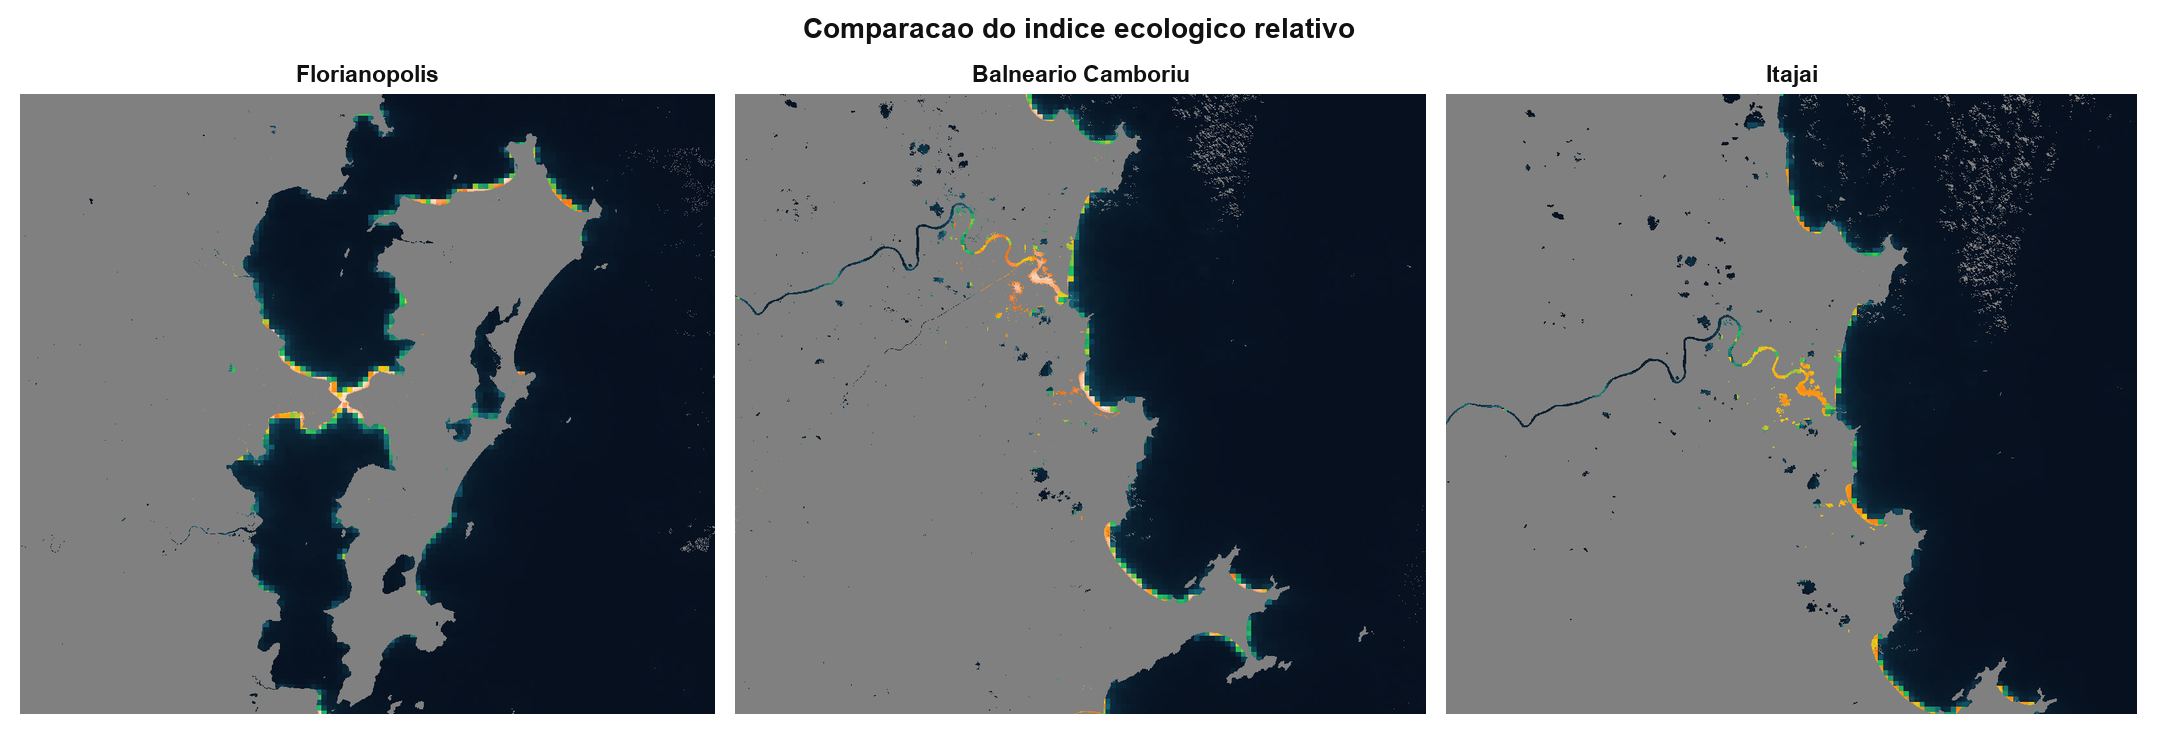
\includegraphics[width=0.95\textwidth]{../EcologicalRiskImages/05-comparisons/comparison-cities-ecological-risk-index.png}
\caption{Comparacao do indice ecologico relativo. As areas claras indicam maior coincidencia entre luz artificial, ambiente aquatico e proxies de sensibilidade ecologica.}
\label{fig:risk}
\end{figure}

Os testes realizados incluiram compilacao dos scripts Python, execucao completa do pipeline, verificacao de imagens nao vazias e conferencias no CSV de metricas. No estado final, foram gerados 22 PNGs em \texttt{EcologicalRiskImages}, sem imagens vazias, tres arrays de produtividade e 10 linhas de metricas para as cidades e buffers analisados.

\subsection{Camadas ambientais e unidades de conservacao}

Para fortalecer a interpretacao ecologica, a Prioridade 3 incluiu duas novas fontes. A primeira e a produtividade primaria. O script \texttt{fetch\_chlorophyll\_data.py} tenta obter clorofila-a em servidores ERDDAP/NOAA. Quando a rede ou o dado nao esta disponivel, o script gera uma camada local reprodutivel, derivada da mascara de agua e da proximidade da costa. Essa decisao garante que o pipeline continue executavel e que a origem da camada fique documentada em \texttt{chlorophyll\_sources.csv}.

\begin{figure}[ht]
\centering
\begin{minipage}{0.32\textwidth}
\centering
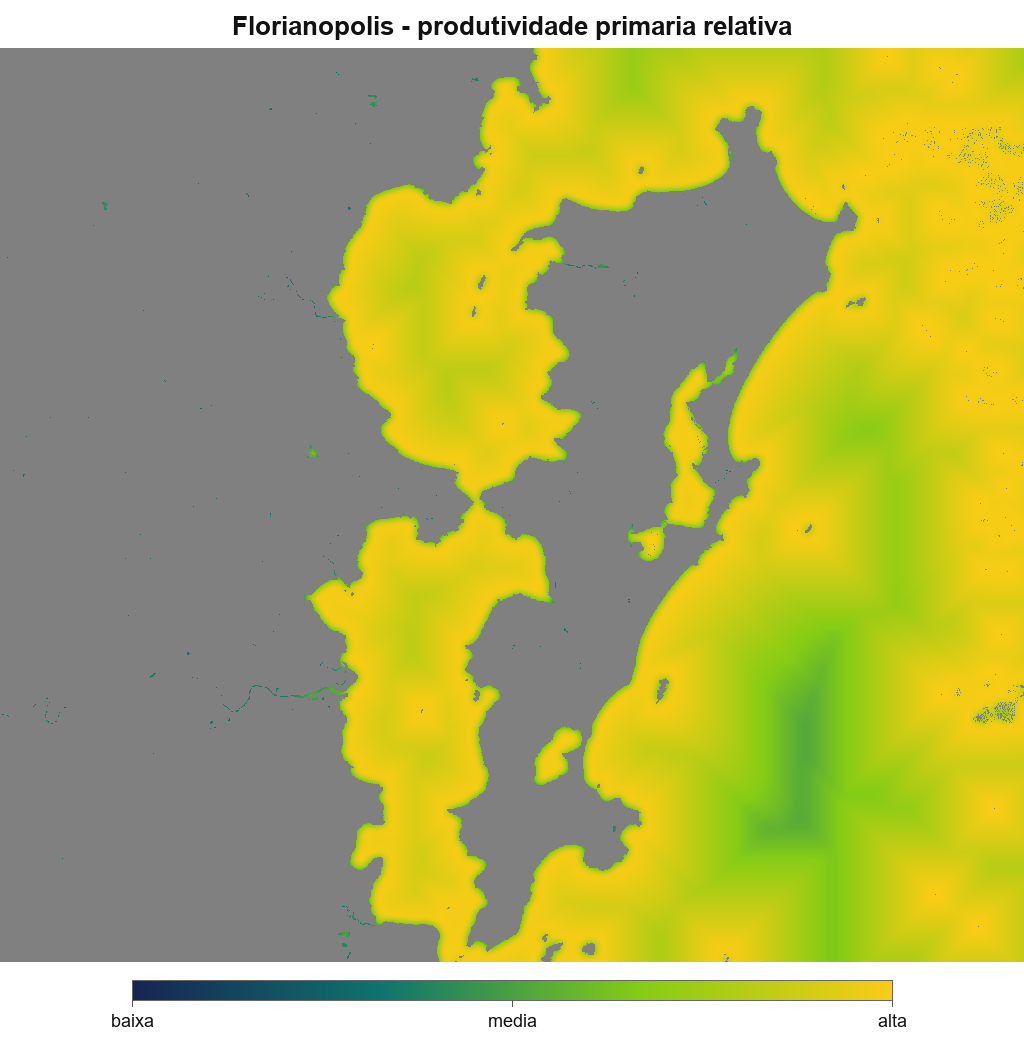
\includegraphics[width=\textwidth]{../EcologicalRiskImages/03-habitat-and-bottom-light/florianopolis-productivity-proxy.png}\\
{\small Produtividade}
\end{minipage}
\begin{minipage}{0.32\textwidth}
\centering
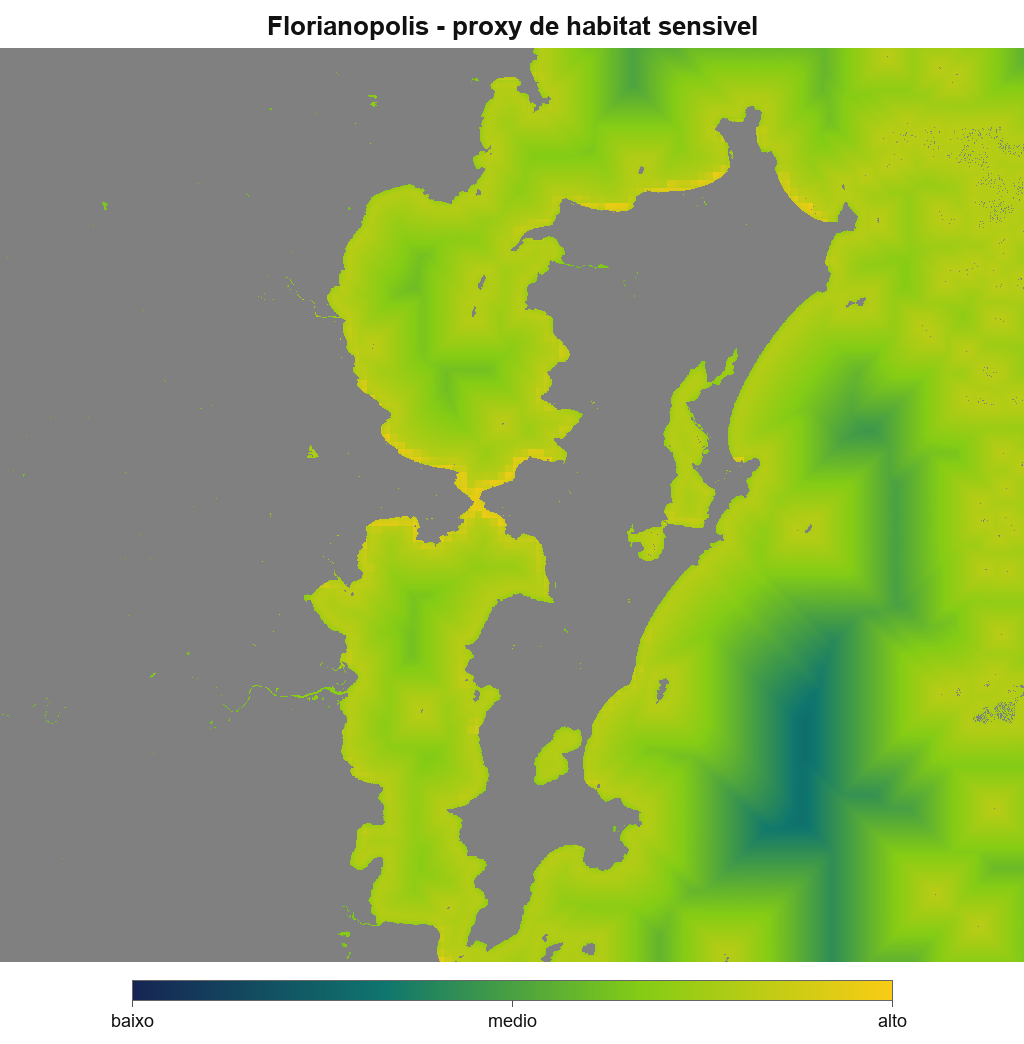
\includegraphics[width=\textwidth]{../EcologicalRiskImages/03-habitat-and-bottom-light/florianopolis-habitat-proxy.png}\\
{\small Habitat}
\end{minipage}
\begin{minipage}{0.32\textwidth}
\centering
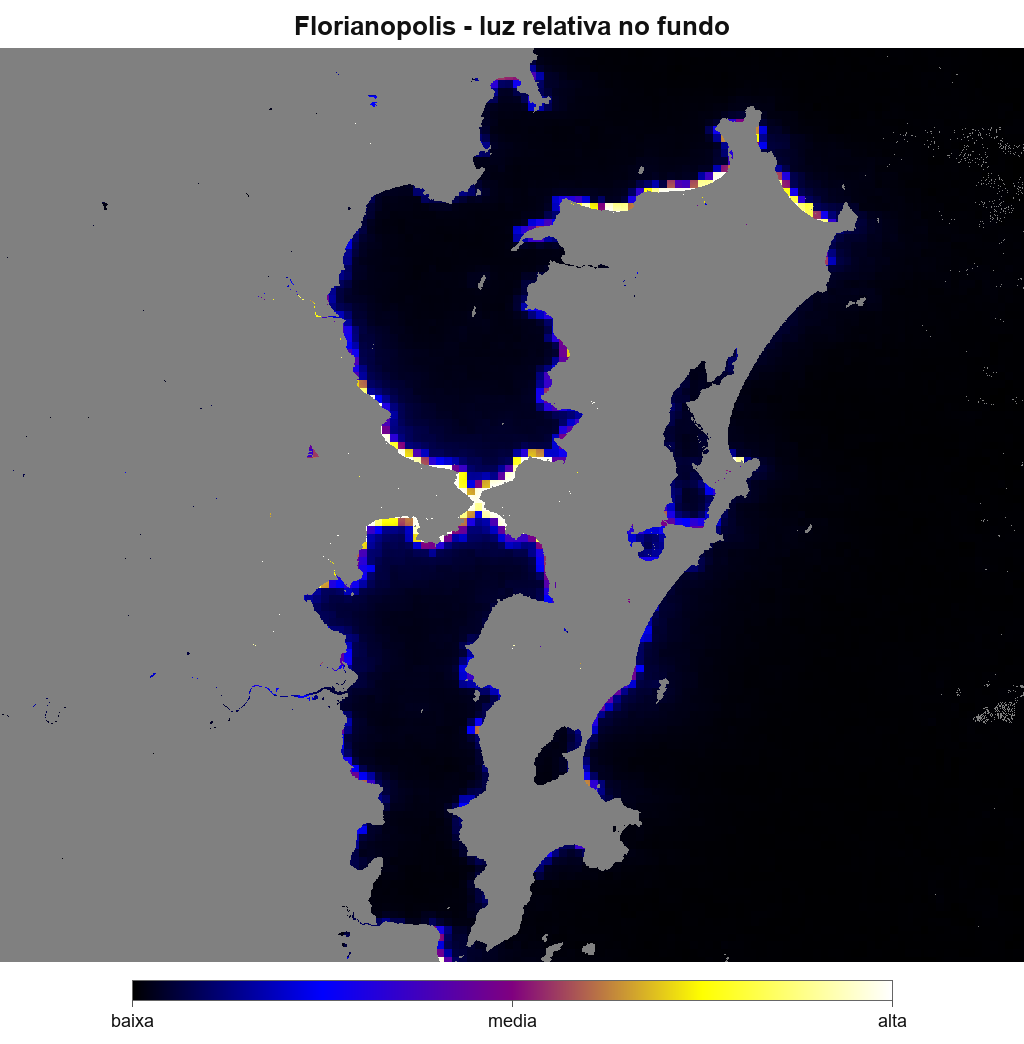
\includegraphics[width=\textwidth]{../EcologicalRiskImages/03-habitat-and-bottom-light/florianopolis-bottom-light-proxy.png}\\
{\small Luz no fundo}
\end{minipage}
\caption{Exemplo de camadas intermediarias para Florianopolis. Elas mostram como o indice final resulta da combinacao entre produtividade, habitat sensivel e luz que permanece relevante em aguas rasas.}
\label{fig:layers}
\end{figure}

A segunda fonte e a sobreposicao com unidades de conservacao. O modulo de sobreposicao carrega um catalogo CSV local na pasta de dados ambientais. Se um GeoJSON externo for colocado na mesma pasta, por exemplo com limites do CNUC/MMA, ele tem prioridade sobre o CSV. Assim, o trabalho permanece funcional sem internet, mas ja esta preparado para limites vetoriais oficiais.

\begin{figure}[ht]
\centering
\begin{minipage}{0.32\textwidth}
\centering
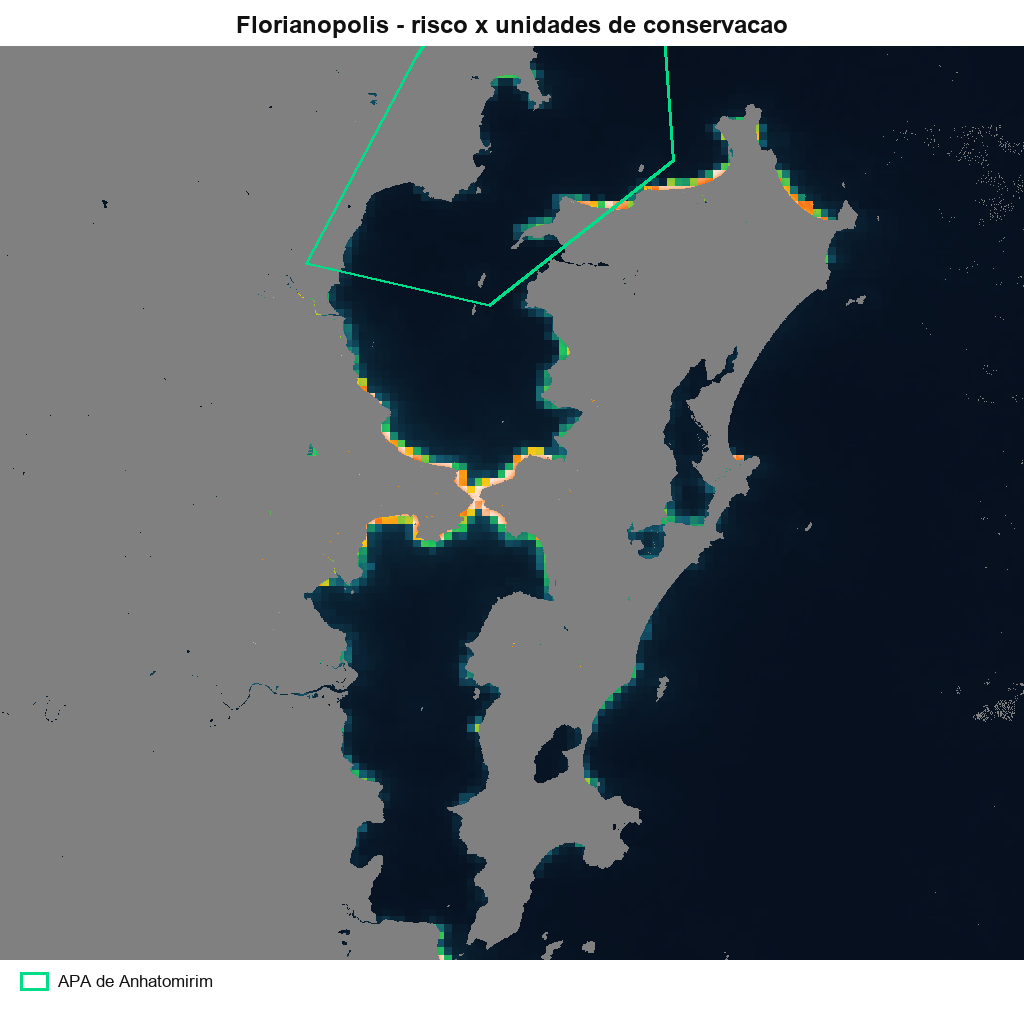
\includegraphics[width=\textwidth]{../EcologicalRiskImages/06-protected-areas/florianopolis-risk-protected-areas.png}\\
{\small Florianopolis}
\end{minipage}
\begin{minipage}{0.32\textwidth}
\centering
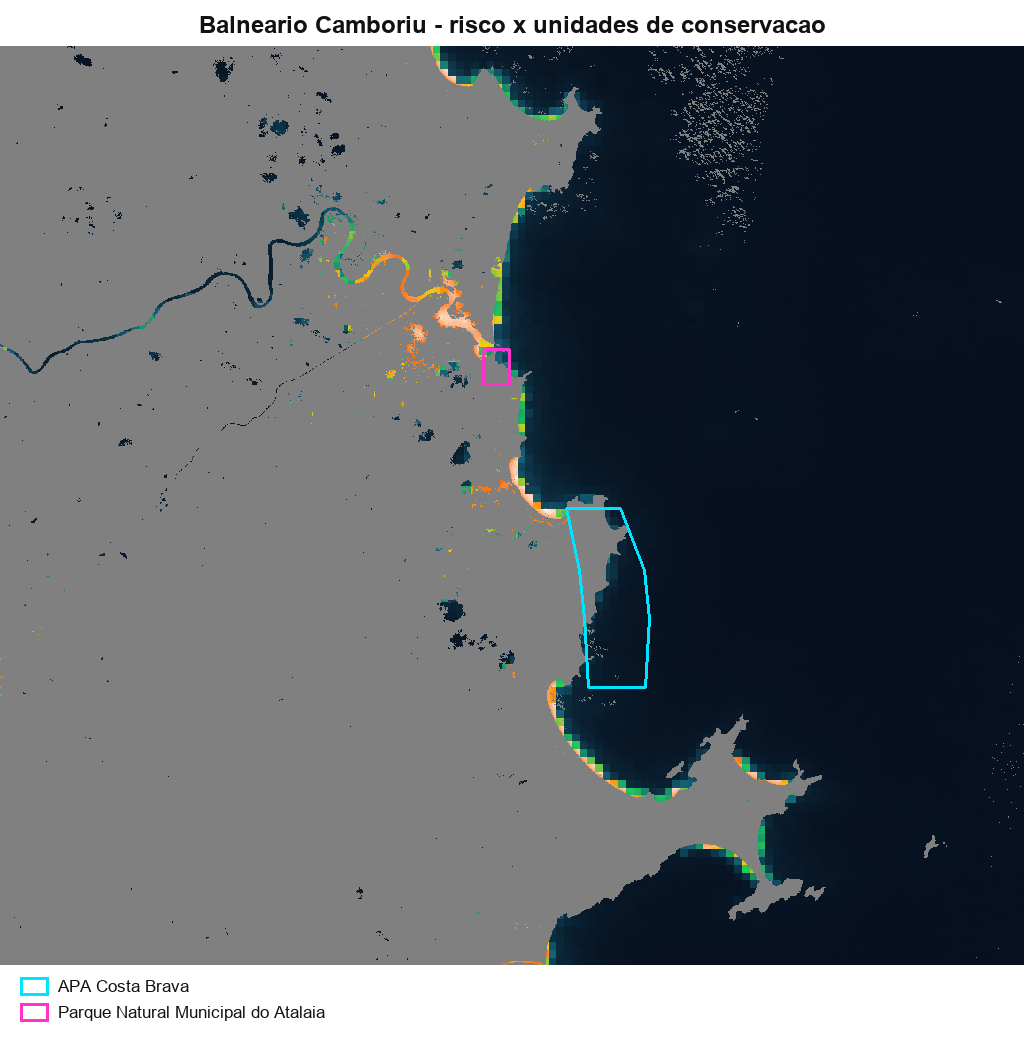
\includegraphics[width=\textwidth]{../EcologicalRiskImages/06-protected-areas/balneario-camboriu-risk-protected-areas.png}\\
{\small Balneario Camboriu}
\end{minipage}
\begin{minipage}{0.32\textwidth}
\centering
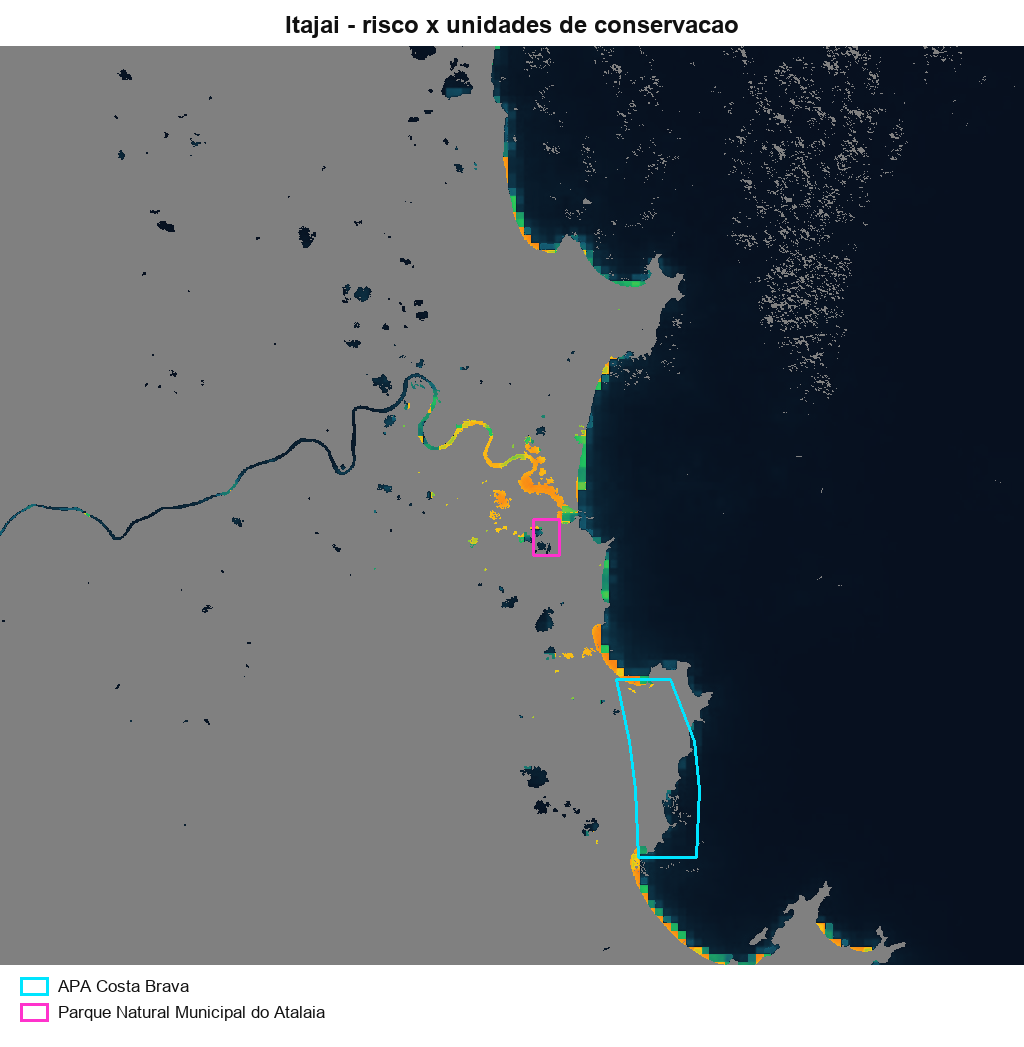
\includegraphics[width=\textwidth]{../EcologicalRiskImages/06-protected-areas/itajai-risk-protected-areas.png}\\
{\small Itajai}
\end{minipage}
\caption{Sobreposicao do risco relativo com unidades de conservacao catalogadas. A figura ajuda a discutir onde areas de risco estimado coincidem com regioes de interesse ambiental.}
\label{fig:protected}
\end{figure}

\section{Resultados e Discussao}

A Tabela~\ref{tab:metrics} apresenta um recorte das metricas finais. Os resultados indicam que o maior risco medio ocorre no buffer de 0--1 km, pois esse intervalo concentra agua costeira rasa, maior influencia urbana e maior intensidade luminosa relativa.

\begin{table}[ht]
\centering
\small
\caption{Metricas principais por cidade e buffer.}
\label{tab:metrics}
\begin{tabular}{|p{3.1cm}|p{1.6cm}|r|r|r|r|}
\hline
Cidade & Buffer & Agua km$^2$ & Luz media & Risco medio & Alto risco km$^2$\\
\hline
Florianopolis & 0--1 km & 542,25 & 0,062 & 0,048 & 9,10\\
Florianopolis & 1--5 km & 709,36 & 0,014 & 0,006 & 0,00\\
Florianopolis & 5--10 km & 65,04 & 0,007 & 0,001 & 0,00\\
Baln. Camboriu & 0--1 km & 357,67 & 0,087 & 0,066 & 12,94\\
Baln. Camboriu & 1--5 km & 653,59 & 0,014 & 0,006 & 0,00\\
Baln. Camboriu & 5--10 km & 201,16 & 0,006 & 0,001 & 0,00\\
Baln. Camboriu & 10--30 km & 10,59 & 0,005 & 0,000 & 0,00\\
Itajai & 0--1 km & 481,98 & 0,062 & 0,038 & 10,48\\
Itajai & 1--5 km & 478,09 & 0,015 & 0,005 & 0,00\\
Itajai & 5--10 km & 147,11 & 0,007 & 0,001 & 0,00\\
\hline
\end{tabular}
\end{table}

Balneario Camboriu apresentou o maior risco medio no buffer de 0--1 km, possivelmente pela forte concentracao de iluminacao na orla urbanizada. Florianopolis apresentou a maior area aquatica analisada nesse mesmo buffer, associada a baiais e ao estreito central. Itajai apresentou concentracao relevante proxima ao canal e a area portuaria. Em todos os casos, a area classificada como alto risco ficou concentrada no primeiro buffer, enquanto os buffers mais distantes apresentaram risco muito baixo.

As figuras mostram que a interpretacao visual e parte essencial do resultado. As mascaras de agua garantem que a analise nao confunda luz urbana com exposicao sobre ambientes aquaticos. Os mapas de produtividade e habitat contextualizam que a camada final nao e apenas uma imagem de brilho. A sobreposicao com unidades de conservacao ajuda a transformar o mapa em uma discussao ambiental, conectando o resultado com areas de gestao e protecao.

\section{Conclusoes}

O trabalho construiu um pipeline completo de processamento de imagem para avaliar poluicao luminosa costeira e risco ecologico relativo em tres cidades de Santa Catarina. A solucao gerou mascaras, gradientes, buffers, metricas tabulares, mapas intermediarios, indice final e sobreposicoes com unidades de conservacao. A principal decisao tecnica foi substituir uma rede neural supervisionada por um classificador deterministico e explicavel, pois nao havia base rotulada suficiente para treinamento robusto.

Os resultados indicam que as regioes mais proximas da costa concentram maior risco relativo. Balneario Camboriu se destaca pelo maior risco medio no buffer imediato, Florianopolis pela extensao de agua exposta e Itajai pela concentracao em torno da area portuaria e canal do Itajai-Acu. Esses achados sao coerentes com a configuracao urbana e costeira das cidades, mas devem ser lidos como indicios relativos, nao como prova de impacto biologico direto.

As principais dificuldades foram a falta de rotulos para treinamento supervisionado, a ausencia de batimetria e coeficientes opticos reais no recorte local, a dependencia de servicos externos para clorofila-a e OBIS, e a necessidade de representar limites de unidades de conservacao sem um GeoJSON oficial disponivel localmente. Para contornar esses pontos, foram usados fallbacks documentados e reprodutiveis, sempre preservando a transparencia metodologica.

Como trabalhos futuros, recomenda-se integrar batimetria GEBCO, coeficientes opticos do Bio-ORACLE ou OceanColor, limites vetoriais oficiais do CNUC/MMA e series temporais VIIRS. Outra melhoria relevante seria montar uma base rotulada por especialistas para permitir comparacao entre o pipeline deterministico atual e modelos supervisionados de aprendizado de maquina.

\begin{thebibliography}{9}

\bibitem{viirs}
NOAA. VIIRS Day/Night Band and night lights products. Disponivel em: \url{https://www.noaa.gov/}.

\bibitem{sentinel}
European Space Agency. Sentinel-2 mission and multispectral imagery. Disponivel em: \url{https://sentinel.esa.int/}.

\bibitem{obis}
Ocean Biodiversity Information System. OBIS API and occurrence data. Disponivel em: \url{https://obis.org/}.

\bibitem{snuc}
Brasil. Lei no 9.985, de 18 de julho de 2000. Institui o Sistema Nacional de Unidades de Conservacao da Natureza.

\bibitem{mndwi}
Xu, H. Modification of normalised difference water index (NDWI) to enhance open water features in remotely sensed imagery. \emph{International Journal of Remote Sensing}, 2006.

\end{thebibliography}

\end{document}
